\documentclass[a4paper]{article}

%% Useful packages
\usepackage{amsmath}
\usepackage{graphicx}
\usepackage[colorinlistoftodos]{todonotes}
\usepackage[colorlinks=true, allcolors=black]{hyperref}
\usepackage[fontsize=11pt]{scrextend}
\usepackage{titlesec}
 \usepackage[section]{placeins}

\setlength\parindent{0pt}
\titleformat*{\section}{\Large\bfseries}
\titleformat*{\subsection}{\Large\bfseries}

\title{PowerEnjoy Service - Design Document}

\begin{document}

\begin{titlepage}
\begin{figure}
\centering

\includegraphics[width=0.2\textwidth]{polimi.jpg}
\par
\LARGE Politecnico di Milano
\end{figure}


\maketitle
\textbf{Version 1.1}
\newline

\raggedright
Authors:
\begin{itemize}
	\item Domenico FAVARO (Mat. 837995)
        	\item Matheus FIM (Mat. 876069)
	\item Caio ZULIANI (Mat. 877266)	
\end{itemize}
\raggedleft
Prof. Elisabetta DI NITTO
\thispagestyle{empty}
\end{titlepage}

\tableofcontents
\newpage
 
\section{Introduction}
\subsection{Purpose}
This Design Document serves the purpose to present to all parties interested the description of the structure for the PowerEnjoy Service. It provides documentation of Software, Architecture and other important aspects of Design to help the understanding and development of the System. Every component that is implemented for the System will be explained as well as the purpose they serve to contribute to the fullfilment of all the project Requirements. All strategies and design decisions will be documented as well.
\subsection{Scope}
This Document presents the PowerEnjoy Software Design Description, decisions and key information to be used to communicate the general purpose of the structure to our stakeholders, and serve as detailed documentation for the components of the System for the developers. This Document will not include detailed information on all the tools and protocols that will be used in the development of the System but rather their purpose and functionality inside the PowerEnjoy System. As example, general knowledge of the Client-Server structure is expected as it will not be rigorously explained but instead how such structure will be used to satisfy our System's Requirements. 
\subsection{Glossary: Definitions, Acronyms, Abbreviations}
\begin{itemize}
\item \textbf{First-Time User:}
\end{itemize}

\subsection{Reference Documents}
\begin{itemize}
\item Specification Document: Assignments AA 2016-2017.pdf
\item PowerEnjoy Requirements And Specifications Document (RASD)
\item IEEE Std 1016-2009 IEEE Standard for Information Technology-Systems Designs-Software Design Descriptions (SDD IEEE 1016-2009.pdf)
\item Example Documents:
\begin{itemize}
\item[-] Remote-Controlled Dissolved Oxygen Monitoring System  (fett\_student\_application\_paper.pdf)
\item[-] Software Design Document (SDD) Template (sdd\_template.pdf)
\end{itemize}
\end{itemize}
\subsection{Document Structure}
\begin{description}
\item \textbf{Section 1 - Introduction:} This section provides a general description of the purpose and structure of this Design Document.
\item \textbf{Section 2 - Architectural Design:} This section illustrates a broader to specific view of the components that form part of the System, presenting from the overview of the architecture of the system to a description of how each component will interface inside the structure.
\item \textbf{Section 3 - Algorithm Design:} Important functionalities of the System that require the development of algorithms will be described in this section.  
\item \textbf{Section 4 - User Interface Design:} All details refering to how the User will interface with the System, from the Web Application to the screens inside the Cars will be shown in this section. As well as general mockups of the Graphical User Interface (GUI) screens.
\item \textbf{Section 5 - Requirements Traceability:} In this section is explained how the Design decisions and structure help fulfill the Requirements for the System that were defined in the RASD. 
\item \textbf{Section 6 - Effort Spent:} Detailed record of the hours worked for each member of the team is documented in this section.
\item \textbf{Section 7 - References:} Any reference to additional external sources that can help the better understanding of this Document is documented in this section.
\end{description}

\newpage
\section{Architectural Design}
\subsection{Overview}
\label{sec:propSystem}
Our Proposed System consist in a 3-tier Client-Server Architecture, with web clients for Users and CRM, mobile App clients for Users and the Car interface that will be implemented as a Client as it's external to our Server System. The Server side will consist on a Java EE Server that will implement a Web Tier for Web Clients and a Business Tier that'll communicate directly to the App Clients. The Server will then connect to the Company's Database that'll be located in our EIS Tier.
Project will be developed using a JEE Platform based in a 3-Tier Client/Server Architecture. First idea consists in a Distributed Logic structured layers where the Client Apps will interface with the Server that will store the logic and will connect with the Data Layer of the System. The architecture as explained briefly in the \textbf{\hyperref[sec:propSystem]{Proposed System}} section will consist of:
\begin {itemize}
\item Client Tier: 
\begin {itemize}
\item [-]Web Client on a browser with abilitated JavaScript for the Web App use. 
\item [-]Application Client for the Mobile App (Android and iOS), with GPS functionalities. We will consider the screen present in the Car as a Client App of the System that'll implement some logic to interface to the Car Software to Lock, Unlock, read the Battery level and other functions.
\end{itemize}

\item Server Tier:
\begin {itemize}
\item [-]Web Server that'll answer connections for Web Clients. It will interface with the Application Server.
\item [-]JavaEE Application Server, that'll implement the logic of the System. Application Clients (Users and Cars) will connect directly to it. Will implement JavaBeans to handle request from multiple Clients at a time.
\end{itemize}

\item Enterprise Information System (EIS) Tier:
\begin{itemize}
\item [-]DataBase Server, accessed by the Application Server to store all the data refering to the System.
\end{itemize}
\end{itemize}

\begin{figure}[h]
\centering
\vspace*{\fill}
\noindent\makebox[\textwidth]{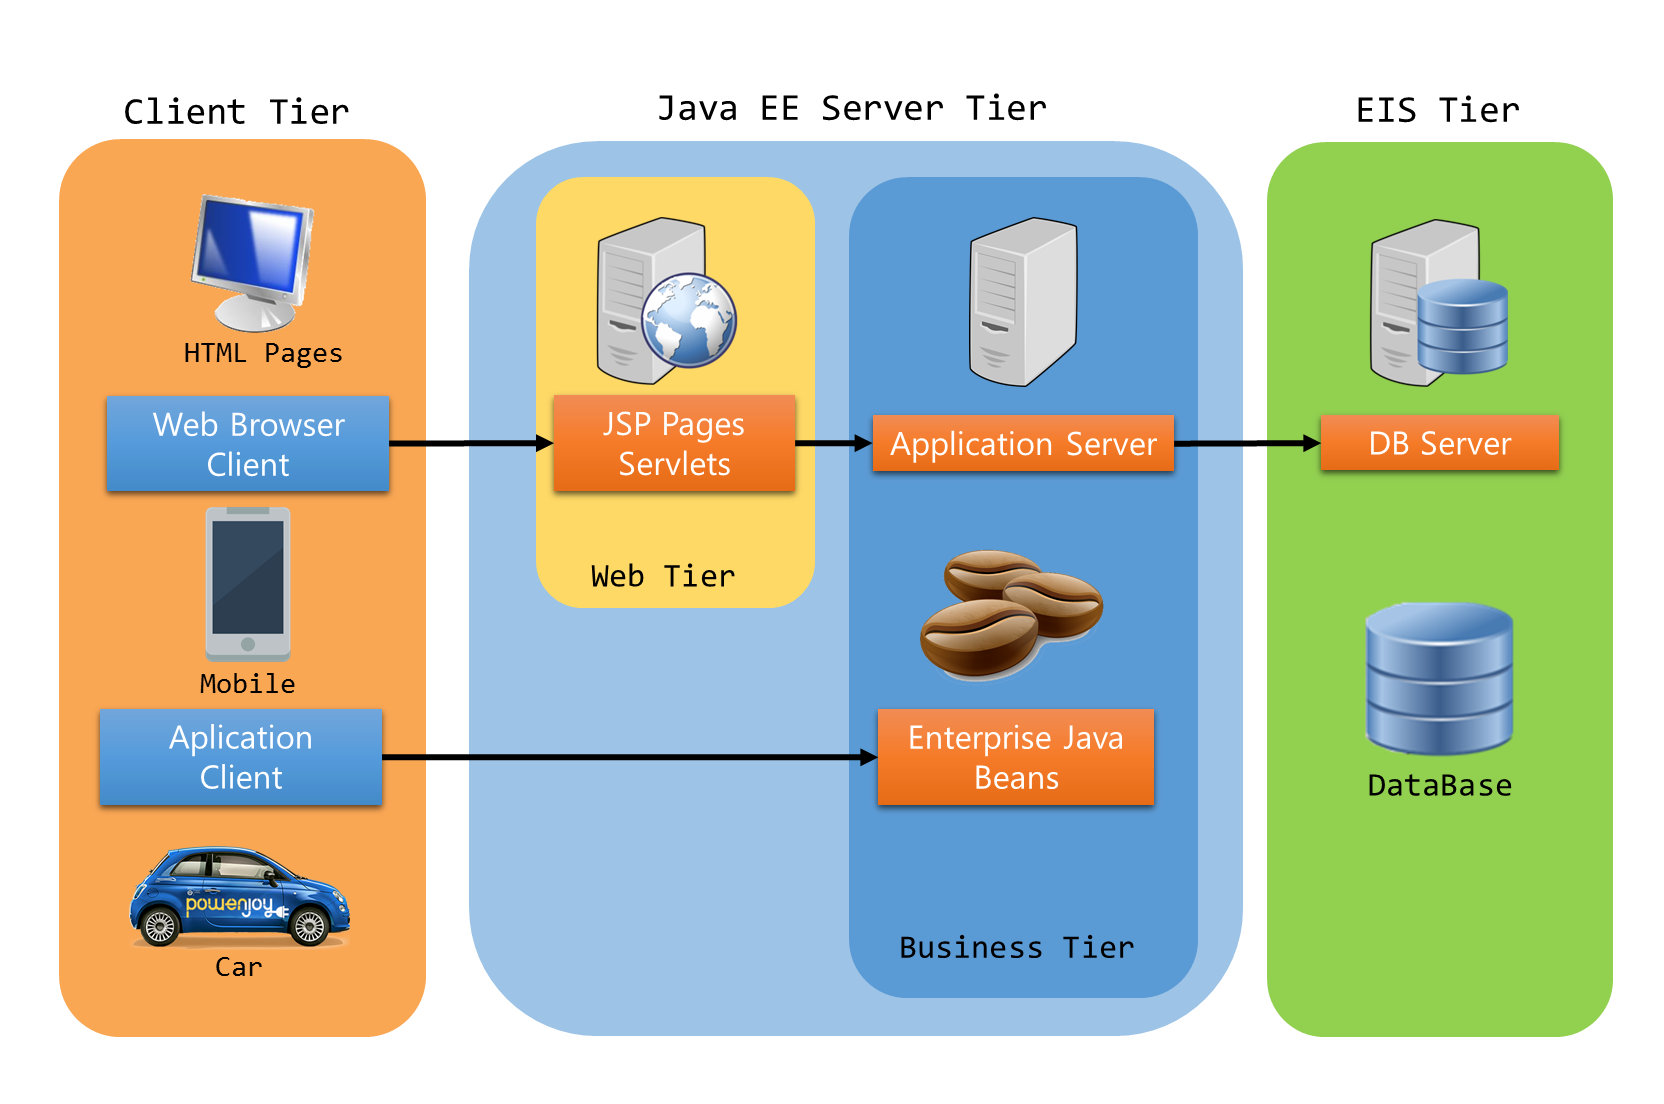
\includegraphics[width=1.35\textwidth]{ProposedSystem.png}}%
\caption {Proposed System Architecture}
\vspace*{0.5cm}
\end{figure}
\newpage

\subsection{Component View}
\subsection{Deployment View}
\subsection{Runtime View}
\subsection{Component Interfaces}
\subsection{Selected Architectural Styles and Patterns}
\subsection{Other Design Decisions}

\section{Algorithm Design}

\section{User Interface Design}
For our User Interface (UI) we'll offer a mobile App for Users and a desktop web App for Users and CRM. They will offer:
\begin {itemize}
\item \textbf{LogIn Page:} First screen of the app with the LogIn and SignIn options.
\begin{figure}[h]
\centering
\vspace*{\fill}
\noindent\makebox[\textwidth]{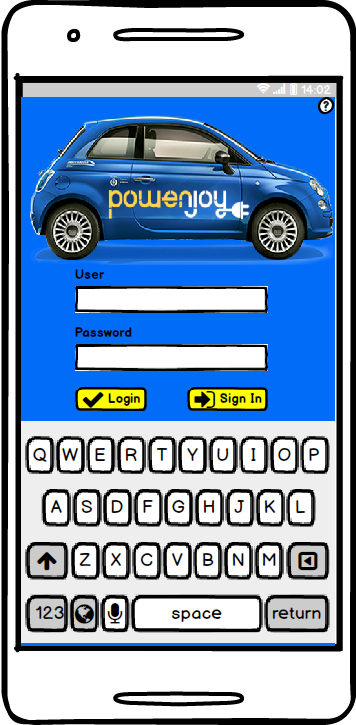
\includegraphics[width=0.28\textwidth]{1.png}}%
\caption {UI LogIn Page}
\vspace*{0.2cm}
\end{figure}
\pagebreak
\item \textbf{Main Page:} Main page of the app where the user sees the map his location and selects the available cars. In Case of CRM, it can see all Cars.
\begin{figure}[h]
\centering
\vspace*{\fill}
\noindent\makebox[\textwidth]{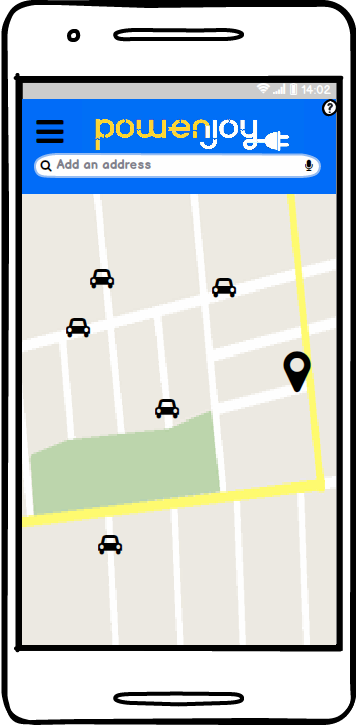
\includegraphics[width=0.28\textwidth]{2.png}}%
\caption {UI Main Page}
\vspace*{0.2cm}
\end{figure}
\item \textbf{Car Details Page:} Once a Car is selected this page allows to reserve a car and contais informations for the decision.
\begin{figure}[h!]
\centering
\vspace*{\fill}
\noindent\makebox[\textwidth]{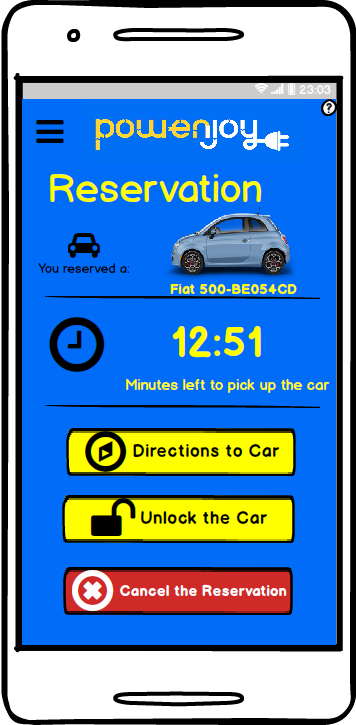
\includegraphics[width=0.28\textwidth]{4.png}}%
\caption {UI Car Details Page}
\vspace*{0.2cm}
\end{figure}
\pagebreak
\item \textbf{Reservation Page:} Once the Reservation is made, the User can see the details of her/his Reservation and have the option to cancel it.
\begin{figure}[h!]
\centering
\vspace*{\fill}
\noindent\makebox[\textwidth]{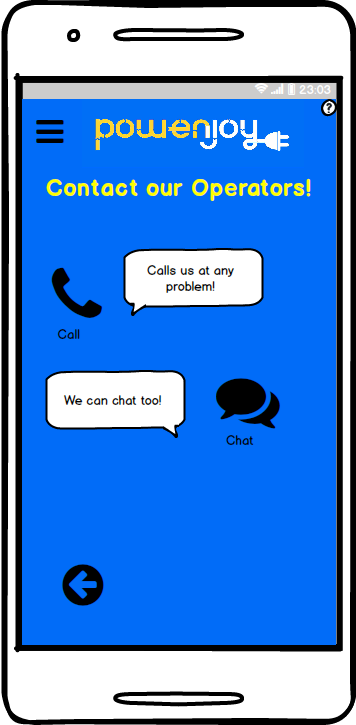
\includegraphics[width=0.28\textwidth]{5.png}}%
\caption {UI Reservation Page}
\vspace*{0.2cm}
\end{figure}
\item \textbf{Ride Page:} Once a Ride started this page shows the details of the current ride, it's present also in the Car screen App.
\begin{figure}[h!]
\centering
\vspace*{\fill}
\noindent\makebox[\textwidth]{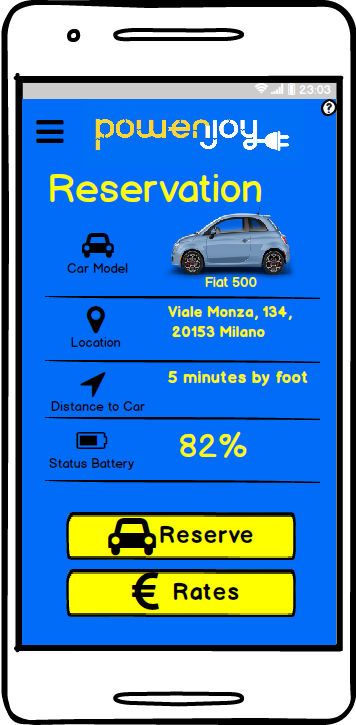
\includegraphics[width=0.36\textwidth]{3.png}}%
\caption {UI Mobile Ride Page}
\vspace*{0.2cm}
\end{figure}
\pagebreak
\begin{figure}[h!]
\centering
\vspace*{\fill}
\noindent\makebox[\textwidth]{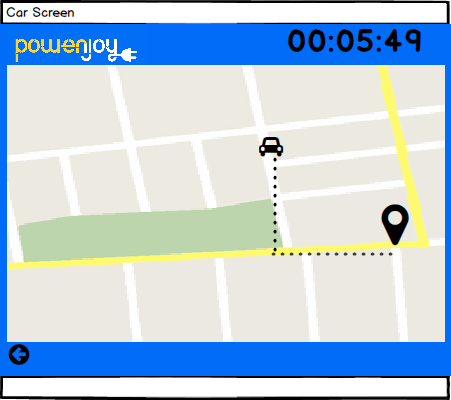
\includegraphics[width=0.7\textwidth]{CarScreen.png}}%
\caption {UI Car Ride Page.}
\vspace*{0.2cm}
\end{figure}
\item \textbf{Email Page:} While not part of the App UI, the System should respond with an email to the User at the end of the Ride showing the final details for it.
\begin{figure}[h!]
\centering
\vspace*{\fill}
\noindent\makebox[\textwidth]{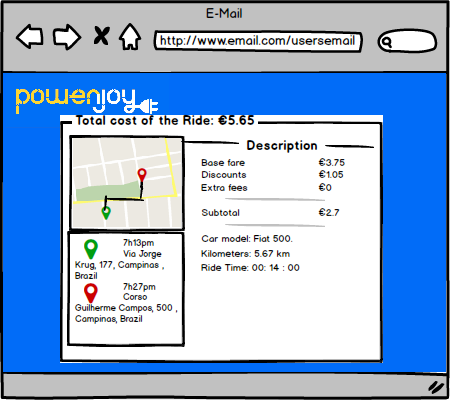
\includegraphics[width=0.7\textwidth]{EmailUser.png}}%
\caption {UI Email Page}
\vspace*{0.2cm}
\end{figure}
\pagebreak
\item \textbf{Contact Page:} Page where the User can contact the CRM operator.
\begin{figure}[h!]
\centering
\vspace*{\fill}
\noindent\makebox[\textwidth]{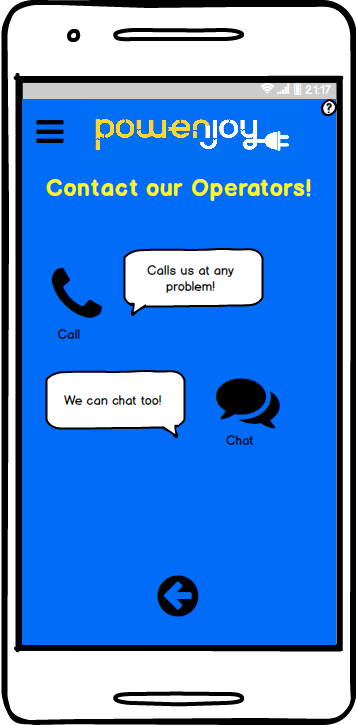
\includegraphics[width=0.28\textwidth]{6.png}}%
\caption {UI Contact Page}
\vspace*{0.2cm}
\end{figure}
\end{itemize}

\section{Requirements Traceability}
\section{Effort Spent}
\begin{tabular}{ | l | l | l | l | }
\hline
	\textbf {Date} & \textbf {Domenico} & \textbf {Caio} & \textbf {Matheus} \\ \hline
	27/11/16& 1h & 1h & 1h  \\ \hline
	28/11/16& 2h & - & - \\ \hline
	29/11/16& - & - & - \\ \hline
	30/11/16& - & - & - \\ \hline
	31/11/16& - & - & - \\ \hline
	01/12/16& - & - & - \\ \hline
	02/12/16& - & - & - \\ \hline
	03/12/16& - & - & - \\ \hline
	04/12/16& - & - & - \\ \hline
	05/12/16& - & - & - \\ \hline
	06/12/16& - & - & - \\ \hline
	07/12/16& - & - & - \\ \hline
	08/12/16& - & - & - \\ \hline
	09/12/16& - & - & - \\ \hline
	10/12/16& - & - & - \\ \hline
	11/12/16& - & - & - \\ \hline
\end{tabular}
\newpage

\section{References}
\newpage


\section{Used Tools}
Keeping track of the Tools used during develop the DD document were:
\begin{itemize}
	\item \textbf{GitHub:} for Version Control
	\item \textbf {Dia Diagram Editor:} for UML Diagrams
	\item \textbf {TeXworks:} for LaTex editing of this Document
\end{itemize}
\newpage

\section{Changelog}
As the project and design decisions may change during the development this document is also prone to change.
We'll document every version in this part.
\begin{itemize}
\item \textbf {Version 1.1:} 11/12/2016
\end{itemize}
\end{document}
